\section{Motivating Example: Smart Grid}
\label{sec:lux-sg-scenario}

\begin{figure*}[ht]
	\centering
    \subfloat[Electricity flow 1] {
		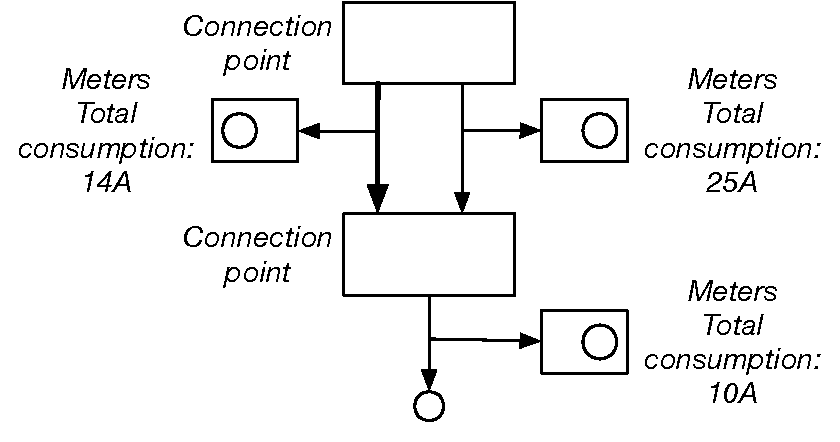
\includegraphics[width=.45\linewidth]{img/chapt-example/duc/Topology1-short}
		\label{fig:intro-schema-topology1}
	}
	\hfill
	\subfloat[Electricity flow 2] {
		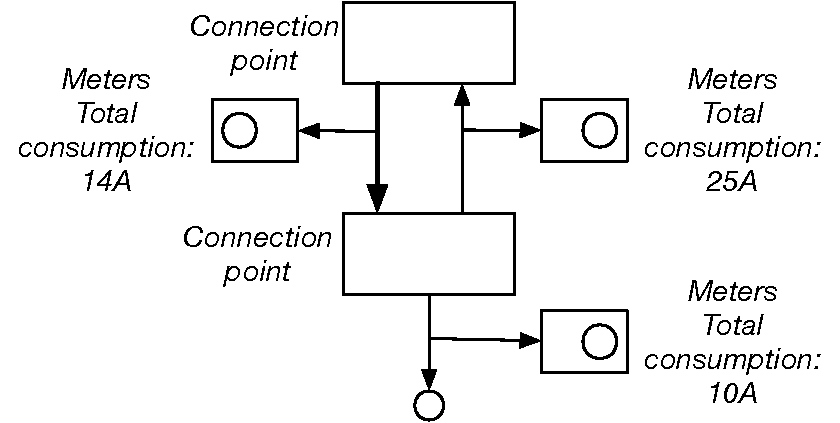
\includegraphics[width=.45\linewidth]{img/chapt-example/duc/Topology2-short}
		\label{fig:intro-schema-topology2}
	}
	\caption{Two different electric flows a same grid topology}
	\label{fig:intro-global}
\end{figure*}

%To exemplify how uncertainty may manifest in programs, we use a smart grid case study, built with Creos Luxembourg, our partner\footnote{Creos Luxembourg is the main grid operator in the country}. 
%More specifically, we focus on cable load estimation and the impacts of not taking uncertain into consideration. 
%We find that this case study is particularly appropriate to exemplify the concepts of uncertainty. 
%We highlight and discuss the limitations of existing approaches when handling such scenarios and show how and when our language is superior to these approaches.

To exemplify how uncertainty may manifest in programs, we use a smart grid case study, built with a partner Creos Luxembourg\footnote{Creos Luxembourg is the main grid operator in the country. \url{https://www.creos-net.lu}}. 
We focus on cable load estimation and the impacts of not taking uncertain into consideration. 
We highlight and discuss the limitations of existing approaches when handling such scenarios.
%Plus, we show how and when our language is superior to these approaches.

\subsection{Overview}
\label{subsec:example-overview}
%The National Institute of Standards and Technology (NIST) defines a smart grid as ``a planned nationwide network that uses information technology to deliver electricity efficiently, reliably, and securely"\footnote{\url{https://www.nist.gov/engineering-laboratory/smart-grid/smart-grid-beginners-guide}}.
%Conceptually, a smart grid is composed of different entities, like smart meters, cabinets (connection points of cables) and power substations.
%These entities are connected, forming a network, and able to exchange information using different technologies~\cite{DBLP:conf/smartgridcomm/0001FKTPTR14, DBLP:conf/sac/0001MFRKT16}.

%The network is the connection linking the smart grid entities by means of physical cables. 
%Every cable has a maximum load depending on its diameter and the used material.
%Figure~\ref{fig:intro-schema-physical} depicts an example of such a network. 
%This network is composed of one substation, one cabinet, and an arbitrary number of smart meters.
%Every cable has two fuses (to connect or disconnect the cable), one at each endpoint.
%By opening or closing fuses, one can influence the electricity flow through the network.
%Figure~\ref{fig:intro-schema-topology1} and~\ref{fig:intro-schema-topology2} show two possible electricity flows over the same physical network, illustrated in Figure~\ref{fig:intro-schema-physical}. 
%We depict closed fuses in black and the direction of the electricity flow using black arrows.

%Smart meters continuously measure electricity consumption and periodically report it to a central data centre.
%Based on this information, together with the grid topology, the electric load of cables can be computed.
%For example, the load on cable endpoint $i_1$ is equal to $\frac{iL_1 + iL_2 + iL_3}{2}$ in the first configuration and to $iL_1 + iL_2 + iL_3$ in the second one.
%With just one difference in one fuse state, there is a factor 2 of the load on $i_1$ between the two situations.
%If the reader wants to go more into the details of the calculation made, we invite him or her to read~\cite{DBLP:conf/sac/0001MFRKT16}.


Conceptually, a smart grid is a graph where the nodes represent the different entities (like meters, connection points of cables) and the edges represent physical cables.
Every cable has two fuses (to connect or disconnect the cable), one at each endpoint.
By opening or closing fuses, one can influence the electricity flow through the network.
Based on this flow and the electricity consumption, the grid manager can estimate the load in every cable.
This computation is detailed in~\cite{DBLP:conf/sac/0001MFRKT16}.

The flow has a big impact on the load cables.
In \autoref{fig:intro-global}, we depict two different flows for the same grid topology.
In both cases, the measured electric consumption are equal.
However, in \autoref{fig:intro-schema-topology1} the load on the left cable (thick line) equals $\frac{14 + 25 + 10}{2} = 24.5$ whereas it equals $14+25+10=49$ in \autoref{fig:intro-schema-topology2}.


\subsection{Impacts of ignoring data uncertainty} 
\label{subsec:example-possible-consequences}
%Although power grids are becoming more and more automated, today human interventions are still the norm.
%For example, most fuses inside cabinets or substations are manually modified by technicians rather than automatically reconfigured.
%As a consequence, the states of fuses are manually documented by technicians on the field. 
%This of course results in mistakes. 
%One way to address this problem is to take uncertainty into consideration.
%This means considering fuse states as uncertain.
%
%As a consequence, this uncertainty propagates to the load calculation formulas, which depend on the fuse states.
%We call this type of uncertainty \textit{uncertain discrete number}. 
%It also propagates to the final load.
%We refer to these values as \textit{uncertain continuous numbers}. 
%In other words, if the uncertainty of fuse states is not considered, it exists a non-null probability that the observed phenomenon does not reflect the real situation.
%Cable load approximations are used to detect cable overloads and to reconfigure the network if necessary.
%By not considering uncertainty, wrong reconfigurations might be triggered, which could be even worse than if no change would have been applied.
%
%In order to model the electricity flow, we can first use a structure or a class to abstract entities (meter, substation, etc.).
%Then, it can be abstracted by linking different entities.
%For example, the substation in Figure~\ref{fig:intro-schema-topology1} contains two references to the cabinet.
%These references are uncertain due to the uncertain nature of fuse states.
%We refer to these references as \textit{uncertain references}.

Although power grids are becoming more and more automated, today human interventions are still the norm.
For example, most fuses are manually modified by technicians rather than automatically reconfigured.
The states of fuses are thus manually documented by technicians on the field. 
This of course results in mistakes. 
One way to address this problem is to take uncertainty into consideration.
This means considering fuse states as uncertain.

As a consequence, this uncertainty propagates to the load calculation formulas, which depend on the fuse states.
If the uncertainty of fuse states is not considered, it exists a non-null probability that the observed phenomenon does not reflect the real situation.
For example, as we have seen in the previous subsection, a modification of the electricity flow may impact the load of a cable with a factor of 2.
Cable load approximations are used to detect cable overloads and to reconfigure the network if necessary.
By not considering uncertainty, wrong reconfigurations might be triggered, which could worsen the situation.

\subsection{Managing uncertainty is not effortless}
In the following, we describe how uncertainty is commonly handled by application developers using current state-of-the-art approaches. 
We show, through code samples, the limitations of these approaches and why we think that these limitations can be addressed by integrating uncertainty management directly at the language level.
In the code excerpts below, we compute the average cable load over the whole grid based on uncertain cable loads. 
A complete version can be found on the GitHub repository. 
All codes contain at least two classes: \textit{SmartGrid} and \textit{Cable}.
The former contains two fields: an array of Cables named \textit{cables} and a function to compute the average load of cables, named \textit{compute\_avg\_load}.
The latter contains one field: an uncertain number which represents the uncertain load.

\paragraph{Manual implementation} 
%One approach for managing uncertainty is to manually implement all the required features.
%Listing~\ref{lst:example-from-scratch} illustrates this (in Python).
%The excerpt contains three classes, UNumber (lines 1--21), SmartGrid (lines 23--31), and Cable (lines 33--35).
%
%As we can see, this approach comes with several drawbacks.
%First, developers are required to have deep knowledge of probability theory.
%For example, uncertainty can be represented by a normal distribution identified by its mean and variance as shown in the constructor ($\_\_init\_\_$), lines 3 and 4.
%One needs knowledge on how to represent it, how to add two normal distributions, ...
%This type is used in the constructor of the class \textit{Cable} to initialize the cable load (line 28).
%In order to support uncertainty propagation through arithmetic operations, one can think of overloading existing arithmetic operations or defining new ones. 
%Languages like Python and C\# allow operator overloading.
%The method definitions $\_\_plus\_\_$ and $\_\_div\_\_$ overload the '+'  and '/' operations respectively. 
%These operators are later used in the SmartGrid class definition to compute the average load, lines 23 and 25.
%
%Second, manual implementation inevitably increases the size of the code base.
%This will de facto augment the risk of errors in the code.
%Plus, the code will be more difficult to maintain afterwards.
%
%Third, although some languages offer the possibility to overload operators, some typing errors can only be detected at runtime. 
%For instance, since Python is dynamically typed, performing an addition operation between \textit{UNumber} and an \textit{UBoolean} fails and raises an exception only at runtime.
%Whilst, statically typed languages such as C\# can detect such typing errors at development time. 
%Nonetheless, the returned exception message would not be particularly meaningful, as can be seen on the example of  C\#: \textit{Operator `+' cannot be applied to operands of type UNumber and UBoolean}. 
%Handling uncertainty at the language-level and extending the typing system, would significantly improve developers' experience and make it possible to detect typing errors at early stages.

One approach for managing uncertainty is to manually implement all the required features.
Listing~\ref{lst:example-from-scratch} illustrates this in Python.
In addition to the \textit{SmartGrid} and \textit{Cable} class, the excerpt contains an additional one: \textit{UNumber}.

As we can see, this approach comes with several drawbacks.
First, developers are required to have deep knowledge of probability theory.
For example, uncertainty can be represented by a normal distribution identified by its mean and variance as shown in the constructor (\textit{\_\_init\_\_}), line 2.
One needs knowledge on how to represent it, how to add two normal distributions, etc.
For example, here we overload the sum and the division operators for two normal distributions (\textit{\_\_plus\_\_} and \textit{\_\_div\_\_} methods).

Second, manual implementation inevitably increases the size of the code base.
This will de facto augment the risk of errors in the code.
Plus, the code will be more difficult to maintain afterwards.

Third, although some languages offer the possibility to overload operators, some typing errors can only be detected at runtime. 
For instance, since Python is dynamically typed, performing an addition operation between two types of uncertain numbers (\ie represented by two classes) fails and raises an exception only at runtime.
Whilst, statically typed languages such as C\# can detect such typing errors at development time. 
Nonetheless, the returned exception message would not be particularly meaningful, as can be seen on the example of  C\#: \textit{Operator `+' cannot be applied to operands of type UNumber1 and UNumber2}.

%\begin{lstlisting}[style=pythonStyle, caption=Manual management of uncertainty in Python, label=lst:example-from-scratch, linewidth=0.97\textwidth
%]
%class UNumber:
%    def __init__(self, mean=0, variance=0):
%        [...]
%
%    def __add__(self, other):
%       [...] # typing error management + casting other to UNumber if it is a Number
%       return UNumber(self.mean + other.mean, self.variance + other.variance)
%
%    def __div__(self, other):
%       [...] # typing error management + casting other to UNumber if it is a Number
%       value = ((self.mean / other.mean) + 
%             (self.mean * other.variance)) / pow(other.mean, 3)
%       variance = (self.variance / other.mean) +
%             (pow(self.mean, 2) * other.variance) / pow(other.mean, 4)
%       return UNumber(value, variance)
%
%class SmartGrid:
%    def __init__(self):
%        self.cables = []
%
%    def compute_avg_load(self):
%        sum_load = 0
%        for c in self.cables:
%            sum_load += c.load
%        return sum_load / len(self.cables)
%
%class Cable:
%    def __init__(self, id, load=UNumber(0, 0)):
%       [...]
%\end{lstlisting}

\begin{lstlisting}[style=pythonStyle, caption=Manual management of uncertainty in Python, label=lst:example-from-scratch, linewidth=0.97\textwidth
]
class UNumber:
  def __init__(self, mean=0, variance=0):
    [...]
    
  def __add__(self, other):
    [...] # typing error management + casting other to UNumber if it is a Number
    return UNumber(self.mean + other.mean, self.variance + other.variance)
    
  def __div__(self, other):
    [...] # typing error management + casting other to UNumber if it is a Number
    value = ((self.mean/other.mean) + (self.mean*other.variance)) / pow(other.mean, 3)
    variance = (self.variance / other.mean) +
             (pow(self.mean, 2) * other.variance) / pow(other.mean, 4)
    return UNumber(value, variance)

class SmartGrid:
  [...]
  def compute_avg_load(self):
    sum_load = 0
    for c in self.cables:
      sum_load += c.load
    return sum_load / len(self.cables)
    
class Cable:
  def __init__(self, id, load=UNumber(0, 0)):
    [...]
\end{lstlisting}

\paragraph{Using existing libraries for probability theory}
%Since uncertainty management relies on probability theory, another approach is using a library implementing common probability distributions.
%%\footnote{\url{https://docs.scipy.org/doc/scipy/reference/stats.html}}
%Staying in Python, there is a widely used library called SciPy library\footnote{\url{https://www.scipy.org/}} and in particular the \textit{stats} module, defining different probability distributions, e.g. the Bernoulli and the Gaussian distributions (cf. Section~\ref{sec:data-uncertainty}).
%Whereas these libraries are suitable to compute different properties of probability distributions, it remains the responsibility of developers to define how to perform arithmetic operations on distributions.
%Listing~\ref{lst:limit-lib-proba} shows an example of the definition of the\textit{ add\_gaussian} method, responsible for adding up two uncertain numbers represented as Gaussian distributions. 
%
%Using such libraries does not prevent developers to have a deep understanding of the probability theory.
%They have been designed to help them manipulating probability distributions, but they still required knowledge about them.
%For example, as shown in Listing~\ref{lst:limit-lib-proba}, one may access the mean and the variance of a normal distribution.
%However, she or he needs to know how two normal distributions can be added.
%This also increases the code base and thus is prone to errors.
%Finally, as it is a library, typing errors will still remain either detected at runtime or not helpful for developers.
Since uncertainty management relies on probability theory, another approach is using a library implementing common probability distributions.
%\footnote{\url{https://docs.scipy.org/doc/scipy/reference/stats.html}}
Staying in Python, there is a widely used library called SciPy\footnote{\url{https://www.scipy.org/}} and in particular the \textit{stats} module, defining different probability distributions.
Whereas these libraries are suitable to compute different properties of probability distributions, it remains the responsibility of developers to define how to perform arithmetic operations on distributions, as depicted in \autoref{lst:limit-lib-proba}.

Using such libraries does not prevent developers to have a deep understanding of the probability theory.
They have been designed to help them manipulating probability distributions, but they still required knowledge about them.
For example, as shown in Listing~\ref{lst:limit-lib-proba}, one may access the mean and the variance of a normal distribution.
However, she or he needs to know how two normal distributions can be added.
This also increases the code base and thus is prone to errors.
Finally, as it is a library, typing errors will still remain either detected at runtime or not helpful for developers.


%\begin{lstlisting}[style=pythonStyle, caption=Limitation using a probability library (Python), label=lst:limit-lib-proba, linewidth=0.97\textwidth]
%from scipy.stats import norm
%
%def add_gaussian(g1, g2):
%    [...]
%    return norm(g1.mean() + g2.mean(), g1.var() + g2.var())
%
%def div_gaussian(g1, g2):
%   [...]
%
%class SmartGrid:
%    def __init__(self):
%        self.cables = []
%
%    def compute_avg_load(self):
%        sum_load = 0
%        for c in self.cables:
%            sum_load = add_gaussian(sum_load, c.load)
%        return div_gaussian(sum_load, len(self.cables))
%
%class Cable:
%    def __init__(self, id, load=norm(0, 0)):
%        [...]
%\end{lstlisting}

\begin{lstlisting}[style=pythonStyle, caption=Limitation using a probability library (Python), label=lst:limit-lib-proba, linewidth=0.97\textwidth]
from scipy.stats import norm

def add_gaussian(g1, g2):
    [...]
    return norm(g1.mean() + g2.mean(), g1.var() + g2.var())

def div_gaussian(g1, g2):
   [...]

class SmartGrid:
    [...]
    def compute_avg_load(self):
        sum_load = 0
        for c in self.cables:
            sum_load = add_gaussian(sum_load, c.load)
        return div_gaussian(sum_load, len(self.cables))

class Cable:
    def __init__(self, id, load=norm(0, 0)):
        [...]
\end{lstlisting}

\paragraph{Using existing libraries for uncertainty}
%Another commonly used approach is to use existing libraries for data uncertainty.
%For example, in Python, using the \textit{uncertainties~\cite{url:uncertainties} library}, a developer can manipulate uncertain floats using variables of type \textit{ufloat}.
%The uncertainty propagation is handled transparently.
%In Listing~\ref{lst:example-python-uncertainties}, we depict a minimalistic excerpt of the necessary code to compute the mean load using an existing library for data uncertainty.
%Unlike the previous code snippet, this listing contains only two classes, SmartGrid and Cable.
%Moreover, the cable load property initialization uses \textit{ufloat} instead of \textit{UNumber}.
%
%Using a library can tackle the two first drawbacks existing in the previous approach: required knowledge of probability theory and code complexity.
%Indeed, the implementation of the probability theory is encapsulated inside the library.
%Developers will just use it through its API.
%The complexity of the implementation, with the possible errors, are also pushed to the complexity.
%We can argue that the library will be well tested and documented.
%
%However, similarly to the previous example, this approach does not extend the type system.
%If the language relies on a dynamic type system (like in Python), then typing errors are raised only at runtime.
%In any case, raised exceptions are not very meaningful.
%For example, if two distributions are sum whereas the operator has not been overloaded for the input distributions, then the error message will just state this operation is not implemented, without any more information.
Another commonly used approach is to use existing libraries for data uncertainty.
For example, in Python, using the \textit{uncertainties}~\cite{url:uncertainties} library, a developer can manipulate uncertain floats using variables of type \textit{ufloat}.
The uncertainty propagation is handled transparently.
In Listing~\ref{lst:example-python-uncertainties}, we depict the code of the load average computation using this library.
The only difference from the previous code snippet, is the missing of the \textit{UNumber} class, not required anymore, and the use of the \textit{ufloat} type for the cable load variable.

Using a library can tackle the two first drawbacks existing in the previous approach: required knowledge of probability theory and code complexity.
Indeed, the implementation of the probability theory and its complexity are encapsulated inside the library.
We can argue that the library will be well tested and documented.
However, similarly to the previous example, this approach does not extend the type system.\looseness-1
%If the language relies on a dynamic type system (like in Python), then typing errors are raised only at runtime.
%In any case, raised exceptions are not very meaningful.
%For example, if two distributions are sum whereas the operator has not been overloaded for the input distributions, then the error message will just state this operation is not implemented, without any more information.

%\begin{lstlisting}[style=pythonStyle, caption=Managing uncertainty in Python using uncertainties~\cite{url:uncertainties}, label=lst:example-python-uncertainties, linewidth=0.97\textwidth, escapechar=\%]
%from uncertainties import ufloat
%
%class SmartGrid:
%    def __init__(self):
%        self.cables = []
%
%    def compute_avg_load(self):
%        [...] # same as in %\autoref{lst:example-from-scratch}%
%
%class Cable:
%    def __init__(self, p_id, p_load=ufloat(0, 0)):
%        self.id = p_id
%        self.load = p_load
%\end{lstlisting}
\begin{lstlisting}[style=pythonStyle, caption=Managing uncertainty in Python using uncertainties~\cite{url:uncertainties}, label=lst:example-python-uncertainties, linewidth=0.97\textwidth, escapechar=\%]
from uncertainties import ufloat

class SmartGrid:
  def __init__(self):
    self.cables = []

  def compute_avg_load(self):
    [...] # same as in %\autoref{lst:example-from-scratch}%

class Cable:
  def __init__(self, id, load=ufloat(0, 0)):
    [...]
\end{lstlisting}

\paragraph{Using a probability programming framework}
Developers can also use a probabilistic programming framework like Infer.NET~\cite{url:InferNET18} or PyMC3~\cite{DBLP:journals/peerj-cs/SalvatierWF16}.
These frameworks allow defining complex probabilistic models and applying inference algorithms.
Contrary to previously described libraries, these frameworks put an effort to set a proper API.
They can be thought as internal domain-specific languages (DSL)\cite{fowler2010domain}\footnote{Martin Fowler defines a DSL as \textquote{a computer programming language of limited expressiveness focused on a particular domain}\cite{fowler2010domain}. An internal DSL is defined inside a general-purpose language, using only a subset of its concept.}.
In Listing~\ref{lst:limit-proba-prog-fw}, we show how the cable load can be computed using the Infer.NET framework.
This approach exposes probability as a first-class language citizen. 
Hence, developers are expected to manipulate probability distributions and not uncertain data types. 
This framework relies on an inference engine to transparently combine probability distributions.
Using such an approach requires a decent acquaintance with probability theory.
We can assume that they are heavily tested, which limits the number of errors.
Plus, in this framework they map arithmetic operators to the combination of probability distributions: developers do not require to create additional work as with the library approach.
But, as it is not implemented at the language level, the typing system is not extended.
Errors will thus either be raised at runtime or not be helpful for developers.

\begin{lstlisting}[style=cSharpStyle, caption=Limitation using a probability programing framework (C\#), label=lst:limit-proba-prog-fw, linewidth=0.97\textwidth]
public class SmartGit {
  public List<Cable> cables { get; private set; }
  private readonly InferenceEngine inference;

  public Gaussian computeAvgLoad() {
    Variable<double> sum = Variable.GaussianFromMeanAndVariance(0,0).Named("sum");
    int i = 0;
    foreach(Cable c in cables)
      sum = (sum + c.load).Named("sum" + i);
      i++;
    Variable<double> result = (sum / cables.Capacity).Named("AvgLoad");
    return (Gaussian) this.inference.Infer(result);
  }
}

public class Cable {
  public Variable<double> load { get; set; }
}
\end{lstlisting}

\paragraph{Sum-up}
Using state-of-art solutions to manage uncertainty, developers have three possibilities: manual implementation, using existing libraries or using a probability programming framework.
As detailed in this section, these approaches will cope with at least one of these drawbacks: developers require a deep understanding of the probability theory, code base will increases which augments the risk of errors, and the type systems may detect errors at runtime or do not provide helpful messages.

%By enhancing uncertainty management as a first-class language citizen, we cope with these three disadvantages.
%In Figure~\ref{fig:motivation-aintea-overview}, we give an overview of our language, \languageName{}.
%Using our contribution, developers can instantiate uncertain variables (boo-lean, numeric or reference) and combine them using the same operators as they are used to (arithmetic, boolean, comparison).
%Plus, we also define new operators to reason over the uncertainty, or the confidence level, of manipulated variables.
%Finally, the type system will be able to detect errors related to probability distribution manipulation, at compilation time as we choose a static type system, with helpful messages.

%\begin{figure}
%	\centering
%	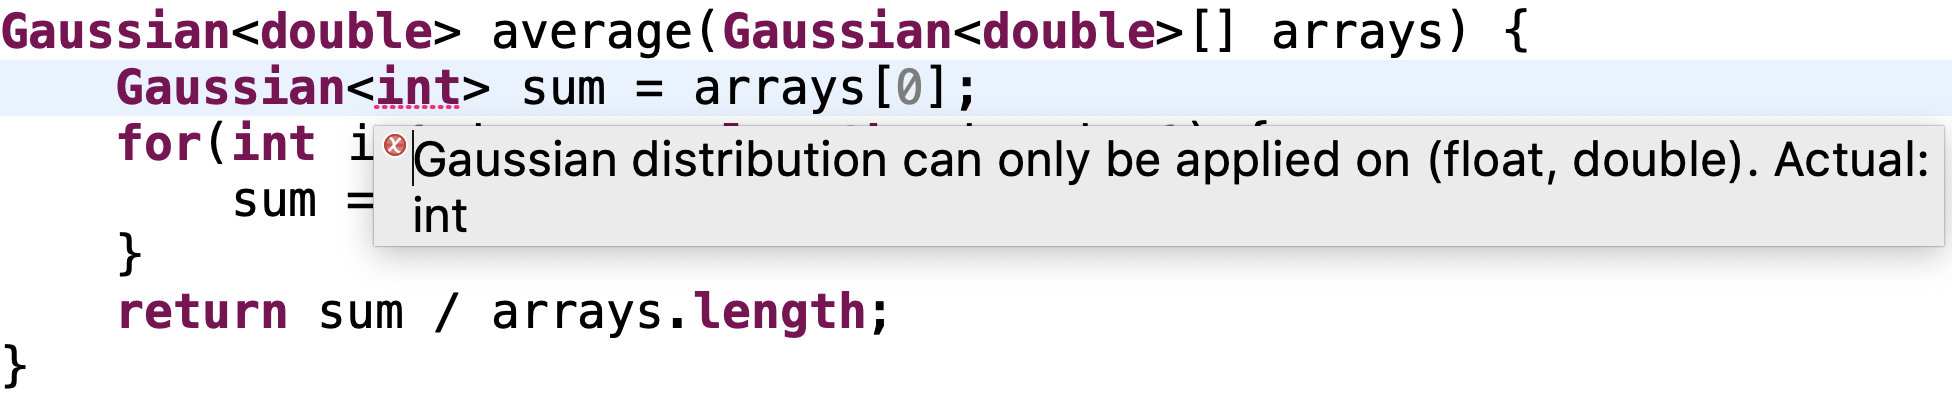
\includegraphics[width=0.6\linewidth]{img/motivation/aintea-overview}
%	\caption{Overview of the language proposed, \languageName{}}
%	\label{fig:motivation-aintea-overview}
%\end{figure}